% This LaTeX was auto-generated from MATLAB code.
% To make changes, update the MATLAB code and export to LaTeX again.

\documentclass{article}

\usepackage[utf8]{inputenc}
\usepackage[T1]{fontenc}
\usepackage{lmodern}
\usepackage{graphicx}
\usepackage{color}
\usepackage{hyperref}
\usepackage{amsmath}
\usepackage{amsfonts}
\usepackage{epstopdf}
\usepackage[table]{xcolor}
\usepackage{matlab}

\sloppy
\epstopdfsetup{outdir=./}
\graphicspath{ {./submission_images/} }

\matlabmultipletitles

\begin{document}

\matlabtitle{ECE1150 ASSIGNMENT7}

\begin{par}
\begin{flushleft}
Yinhao Qian @ University of Pittsburgh
\end{flushleft}
\end{par}


\matlabtitle{Q1}

\begin{matlabcode}
clearvars -except answer;
addrRang_C = {
    {'11100000 00000000 00000000 00000000',
    '11100000 00111111 11111111 11111111'},
    {'11100000 01000000 00000000 00000000',
    '11100000 01000000 11111111 11111111'},
    {'11100000 01000001 00000000 00000000',
    '11100001 01111111 11111111 11111111'}};
for i = 1:1:numel(addrRang_C)
    puts("link interface "+(i-1),'');
    generateForwardingTable(addrRang_C{i}{1}, ...
        addrRang_C{i}{2});
end
\end{matlabcode}
\begin{matlaboutput}
      -> link interface 0
FROM  -> 11100000000000000000000000000000
TO    -> 11100000001111111111111111111111
TABLE -> 11100000000000000000000000000000
RES   -> 224.0.0.0 | 10
      -> link interface 1
FROM  -> 11100000010000000000000000000000
TO    -> 11100000010000001111111111111111
TABLE -> 11100000010000000000000000000000
RES   -> 224.64.0.0 | 16
      -> link interface 2
FROM  -> 11100000010000010000000000000000
TO    -> 11100001011111111111111111111111
TABLE -> 11100000000000000000000000000000
RES   -> 224.0.0.0 | 7
\end{matlaboutput}
\begin{matlabcode}
puts('all others go to link interface 3','');
\end{matlabcode}
\begin{matlaboutput}
      -> all others go to link interface 3
\end{matlaboutput}


\matlabtitle{Q2A}

\begin{matlabcode}
clearvars -except answer;
src = ["138.76.29.7:9001","138.76.29.7:9002","138.76.29.7:9003"];
dest = ["192.168.0.2:1533","192.168.0.3:2202","192.168.0.4:2489"];
dest2src = containers.Map(dest,src);
\end{matlabcode}

\begin{par}
\begin{flushleft}
Source IP: port number Destination IP: port number 192.168.0.3:2202 136.142.34.104:80 192.168.0.4:2489 52.25.108.148:443
\end{flushleft}
\end{par}

\begin{matlabcode}
res = ["192.168.0.3:2202", "136.142.34.104:80";
    "192.168.0.4:2489","52.25.108.148:443"];
\end{matlabcode}

\matlabheading{Original Table:}

\begin{matlabcode}
disp(res);
\end{matlabcode}
\begin{matlaboutput}
    "192.168.0.3:2202"    "136.142.34.104:80"
    "192.168.0.4:2489"    "52.25.108.148:443"
\end{matlaboutput}
\begin{matlabcode}
for i = 1:1:2%NAT translation process
    res(i,1) = convertCharsToStrings( ...
        dest2src(convertStringsToChars(res(i,1))));
end
\end{matlabcode}

\matlabheading{Translated Table:}

\begin{matlabcode}
disp(res)
\end{matlabcode}
\begin{matlaboutput}
    "138.76.29.7:9002"    "136.142.34.104:80"
    "138.76.29.7:9003"    "52.25.108.148:443"
\end{matlaboutput}

\matlabtitle{Q2B}

\begin{matlabcode}
src2dest = containers.Map(src,dest);
req = ["136.142.34.104:80", "138.76.29.7:9003";
    "52.25.108.148:443","138.76.29.7:9002"];
\end{matlabcode}

\matlabheading{Original Table:}

\begin{matlabcode}
disp(req);
\end{matlabcode}
\begin{matlaboutput}
    "136.142.34.104:80"    "138.76.29.7:9003"
    "52.25.108.148:443"    "138.76.29.7:9002"
\end{matlaboutput}
\begin{matlabcode}
for i = 1:1:2%NAT translation process
    req(i,2) = convertCharsToStrings( ...
        src2dest(convertStringsToChars(req(i,2))));
end
\end{matlabcode}

\matlabheading{Translated Table:}

\begin{matlabcode}
disp(req);
\end{matlabcode}
\begin{matlaboutput}
    "136.142.34.104:80"    "192.168.0.4:2489"
    "52.25.108.148:443"    "192.168.0.3:2202"
\end{matlaboutput}


\matlabtitle{Q3}

\begin{matlabcode}
clearvars -except answer;
\end{matlabcode}

\begin{par}
\begin{flushleft}
Reference Table (demostrating known distance information):
\end{flushleft}
\end{par}

\begin{matlabcode}
V = {'x','y','z','u','v'};
x = [0,3,2,inf,3]';
y = [3,0,inf,2,inf]';
z = [2,inf,0,inf,6]';
u = [inf,2,inf,0,1]';
v = [3,inf,6,1,0]';
T_REF = table(x,y,z,u,v,'RowNames',V);
disp(T_REF);
\end{matlabcode}
\begin{matlaboutput}
          x      y      z      u      v 
         ___    ___    ___    ___    ___

    x      0      3      2    Inf      3
    y      3      0    Inf      2    Inf
    z      2    Inf      0    Inf      6
    u    Inf      2    Inf      0      1
    v      3    Inf      6      1      0
\end{matlaboutput}

\begin{par}
\begin{flushleft}
Operating Table (used to calculate the shortest distance):
\end{flushleft}
\end{par}

\begin{matlabcode}
R = {'x','z','v'};
T = table(inf(1,3)',inf(1,3)',inf(1,3)',inf(1,3)',inf(1,3)', ...
    'VariableNames',V,'RowNames',R);
disp(T);
\end{matlabcode}
\begin{matlaboutput}
          x      y      z      u      v 
         ___    ___    ___    ___    ___

    x    Inf    Inf    Inf    Inf    Inf
    z    Inf    Inf    Inf    Inf    Inf
    v    Inf    Inf    Inf    Inf    Inf
\end{matlaboutput}
\begin{matlabcode}
isTableChanged_lA = [true,true,true];
for from = 1:1:numel(R)%from this node
    puts("testing row "+R{from},'row');
    T{R{from},R{from}} = 0;
    while true
        doMadeChanges_l = false;
        for gpas = 1:1:numel(V)%going pass this node   
            for to = 1:1:numel(V)%to this node
                origCost_d = T{R{from},V{to}};
                newCost_d = T{R{from},V{gpas}}
                +T_REF{V{gpas},V{to}};
                if newCost_d<origCost_d
                    doMadeChanges_l = true;
                    puts("from "+R{from} ...
                        +" ,it's less costly to go thru " ...
                        +V{gpas}+" to reach "+V{to} ...
                        +" since "+T{R{from},V{to}}+" > " ...
                        + T{R{from},V{gpas}} ...
                        + " + "+ T_REF{V{gpas},V{to}} ,'');
                    T{R{from},V{to}} = newCost_d;
                    disp(T(from,:))
                end
            end
        end
\end{matlabcode}

\begin{par}
\begin{flushleft}
        Instead of solely having 3 iterations, I'll keep it running until no more changes to the table are made (to show the final result)
\end{flushleft}
\end{par}

\begin{matlabcode}
        if(doMadeChanges_l==false)
            break
        end
    end
end
\end{matlabcode}
\begin{matlaboutput}
ROW   -> testing row x
      -> from x ,it's less costly to go thru x to reach y since Inf > 0 + 3
         x    y     z      u      v 
         _    _    ___    ___    ___

    x    0    3    Inf    Inf    Inf
      -> from x ,it's less costly to go thru x to reach z since Inf > 0 + 2
         x    y    z     u      v 
         _    _    _    ___    ___

    x    0    3    2    Inf    Inf
      -> from x ,it's less costly to go thru x to reach v since Inf > 0 + 3
         x    y    z     u     v
         _    _    _    ___    _

    x    0    3    2    Inf    3
      -> from x ,it's less costly to go thru y to reach u since Inf > 3 + 2
         x    y    z    u    v
         _    _    _    _    _

    x    0    3    2    5    3
      -> from x ,it's less costly to go thru v to reach u since 5 > 3 + 1
         x    y    z    u    v
         _    _    _    _    _

    x    0    3    2    4    3
ROW   -> testing row z
      -> from z ,it's less costly to go thru z to reach x since Inf > 0 + 2
         x     y     z     u      v 
         _    ___    _    ___    ___

    z    2    Inf    0    Inf    Inf
      -> from z ,it's less costly to go thru z to reach v since Inf > 0 + 6
         x     y     z     u     v
         _    ___    _    ___    _

    z    2    Inf    0    Inf    6
      -> from z ,it's less costly to go thru v to reach u since Inf > 6 + 1
         x     y     z    u    v
         _    ___    _    _    _

    z    2    Inf    0    7    6
      -> from z ,it's less costly to go thru x to reach y since Inf > 2 + 3
         x    y    z    u    v
         _    _    _    _    _

    z    2    5    0    7    6
      -> from z ,it's less costly to go thru x to reach v since 6 > 2 + 3
         x    y    z    u    v
         _    _    _    _    _

    z    2    5    0    7    5
      -> from z ,it's less costly to go thru v to reach u since 7 > 5 + 1
         x    y    z    u    v
         _    _    _    _    _

    z    2    5    0    6    5
ROW   -> testing row v
      -> from v ,it's less costly to go thru v to reach x since Inf > 0 + 3
         x     y      z      u     v
         _    ___    ___    ___    _

    v    3    Inf    Inf    Inf    0
      -> from v ,it's less costly to go thru v to reach z since Inf > 0 + 6
         x     y     z     u     v
         _    ___    _    ___    _

    v    3    Inf    6    Inf    0
      -> from v ,it's less costly to go thru v to reach u since Inf > 0 + 1
         x     y     z    u    v
         _    ___    _    _    _

    v    3    Inf    6    1    0
      -> from v ,it's less costly to go thru x to reach y since Inf > 3 + 3
         x    y    z    u    v
         _    _    _    _    _

    v    3    6    6    1    0
      -> from v ,it's less costly to go thru x to reach z since 6 > 3 + 2
         x    y    z    u    v
         _    _    _    _    _

    v    3    6    5    1    0
      -> from v ,it's less costly to go thru u to reach y since 6 > 1 + 2
         x    y    z    u    v
         _    _    _    _    _

    v    3    3    5    1    0
\end{matlaboutput}

\begin{par}
\begin{flushleft}
Final table:
\end{flushleft}
\end{par}

\begin{matlabcode}
disp(T);
\end{matlabcode}
\begin{matlaboutput}
         x    y    z    u    v
         _    _    _    _    _

    x    0    3    2    4    3
    z    2    5    0    6    5
    v    3    3    5    1    0
\end{matlaboutput}


\matlabtitle{Q4}

\begin{par}
\begin{flushleft}
This command presented me withg the resolved MAC addresses saved in cache: 
\end{flushleft}
\end{par}

\begin{par}
\begin{flushleft}
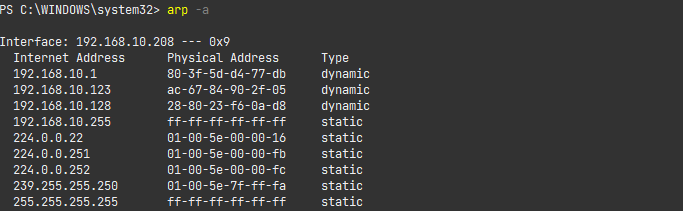
\includegraphics[width=\maxwidth{50.17561465127948em}]{image_0}
\end{flushleft}
\end{par}

\begin{par}
\begin{flushleft}
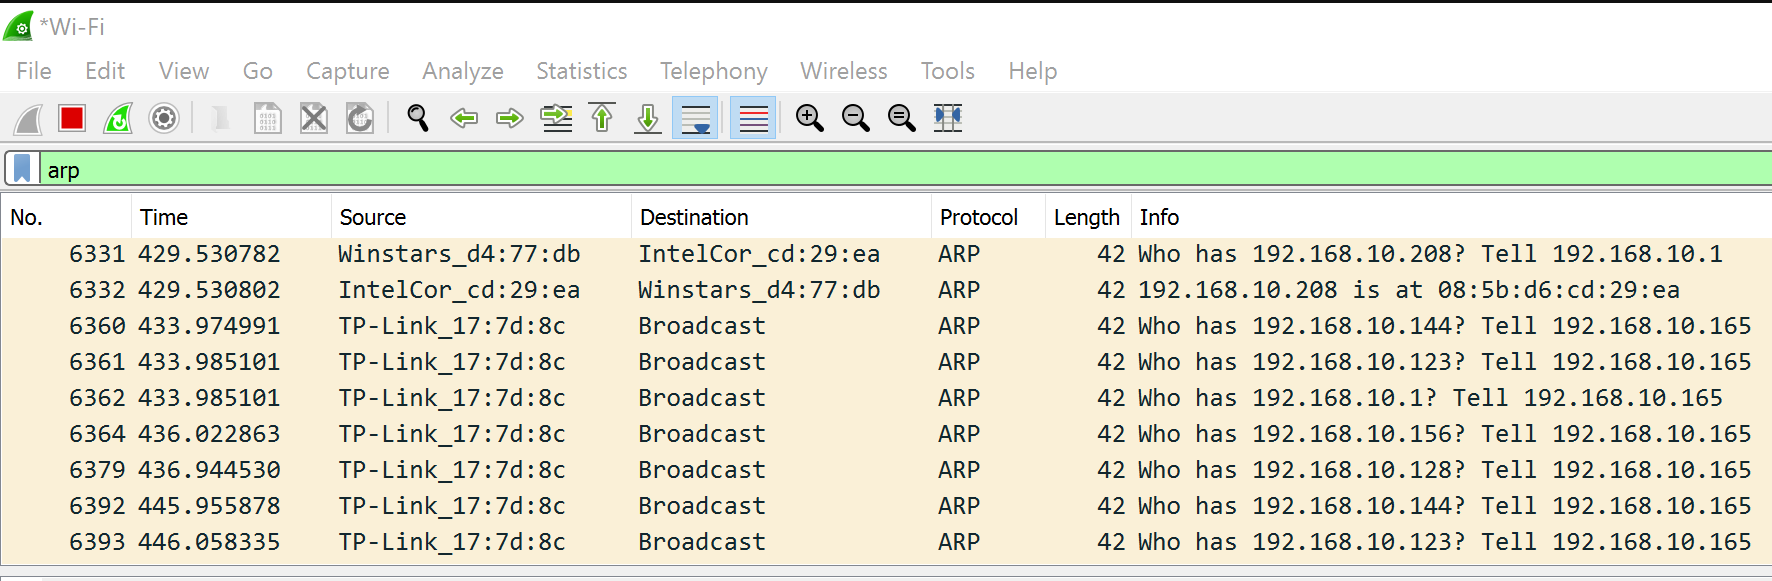
\includegraphics[width=\maxwidth{50.17561465127948em}]{image_1}
\end{flushleft}
\end{par}

\begin{par}
\begin{flushleft}
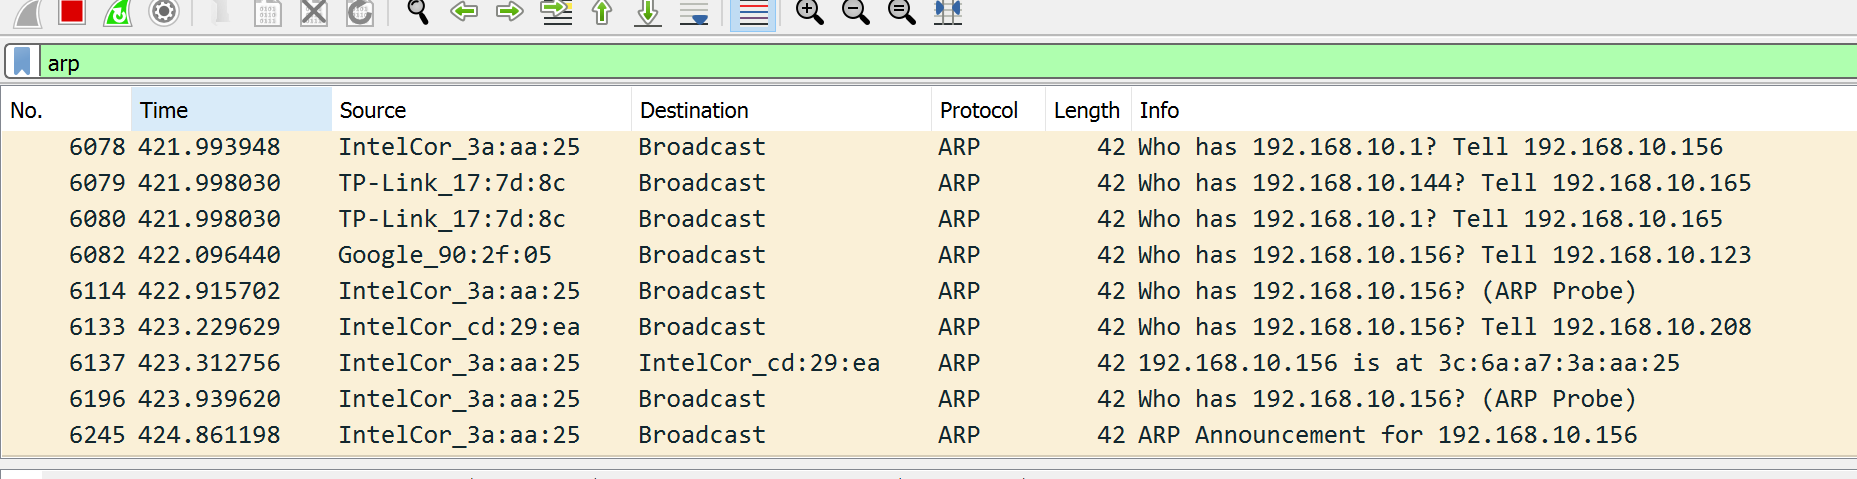
\includegraphics[width=\maxwidth{50.17561465127948em}]{image_2}
\end{flushleft}
\end{par}

\begin{par}
\begin{flushleft}
As we can see, in arp process, both receving and tranmitting uses broadcast rather than unicast. 
\end{flushleft}
\end{par}

\begin{par}
\begin{flushleft}
Unfortunately there are too many servers that requires internet on my device, so it's very difficult to tell which one is for connecting to my.pitt.edu.
\end{flushleft}
\end{par}

\begin{par}
\begin{flushleft}
The purpose of arp messages is that it translates IP addresses and MAC addresses so that devices know what is the actual destination addresses so that they can send packets to each other. 
\end{flushleft}
\end{par}


\matlabtitle{Q5A}

\begin{par}
\begin{flushleft}
Transport Control Protocol aka TCP needs a three way handshake to make sure connection is established before sending data, and error checking is also present in TCP protocol (either stop-and-wait or sliding-window). It's more secure than UDP but slower and takes more resources.
\end{flushleft}
\end{par}

\begin{par}
\begin{flushleft}
User Datagram Protocol aka UDP does not need to establish any connections, and all data is broadcasted and doesn't care it the receiver's reaction. It's easier to use and has less overhead.
\end{flushleft}
\end{par}

\matlabtitle{Q5B}

\begin{par}
\begin{flushleft}
I use Socket.IO for web programming, and it employs TCP protocol.
\end{flushleft}
\end{par}

\begin{par}
\begin{flushleft}
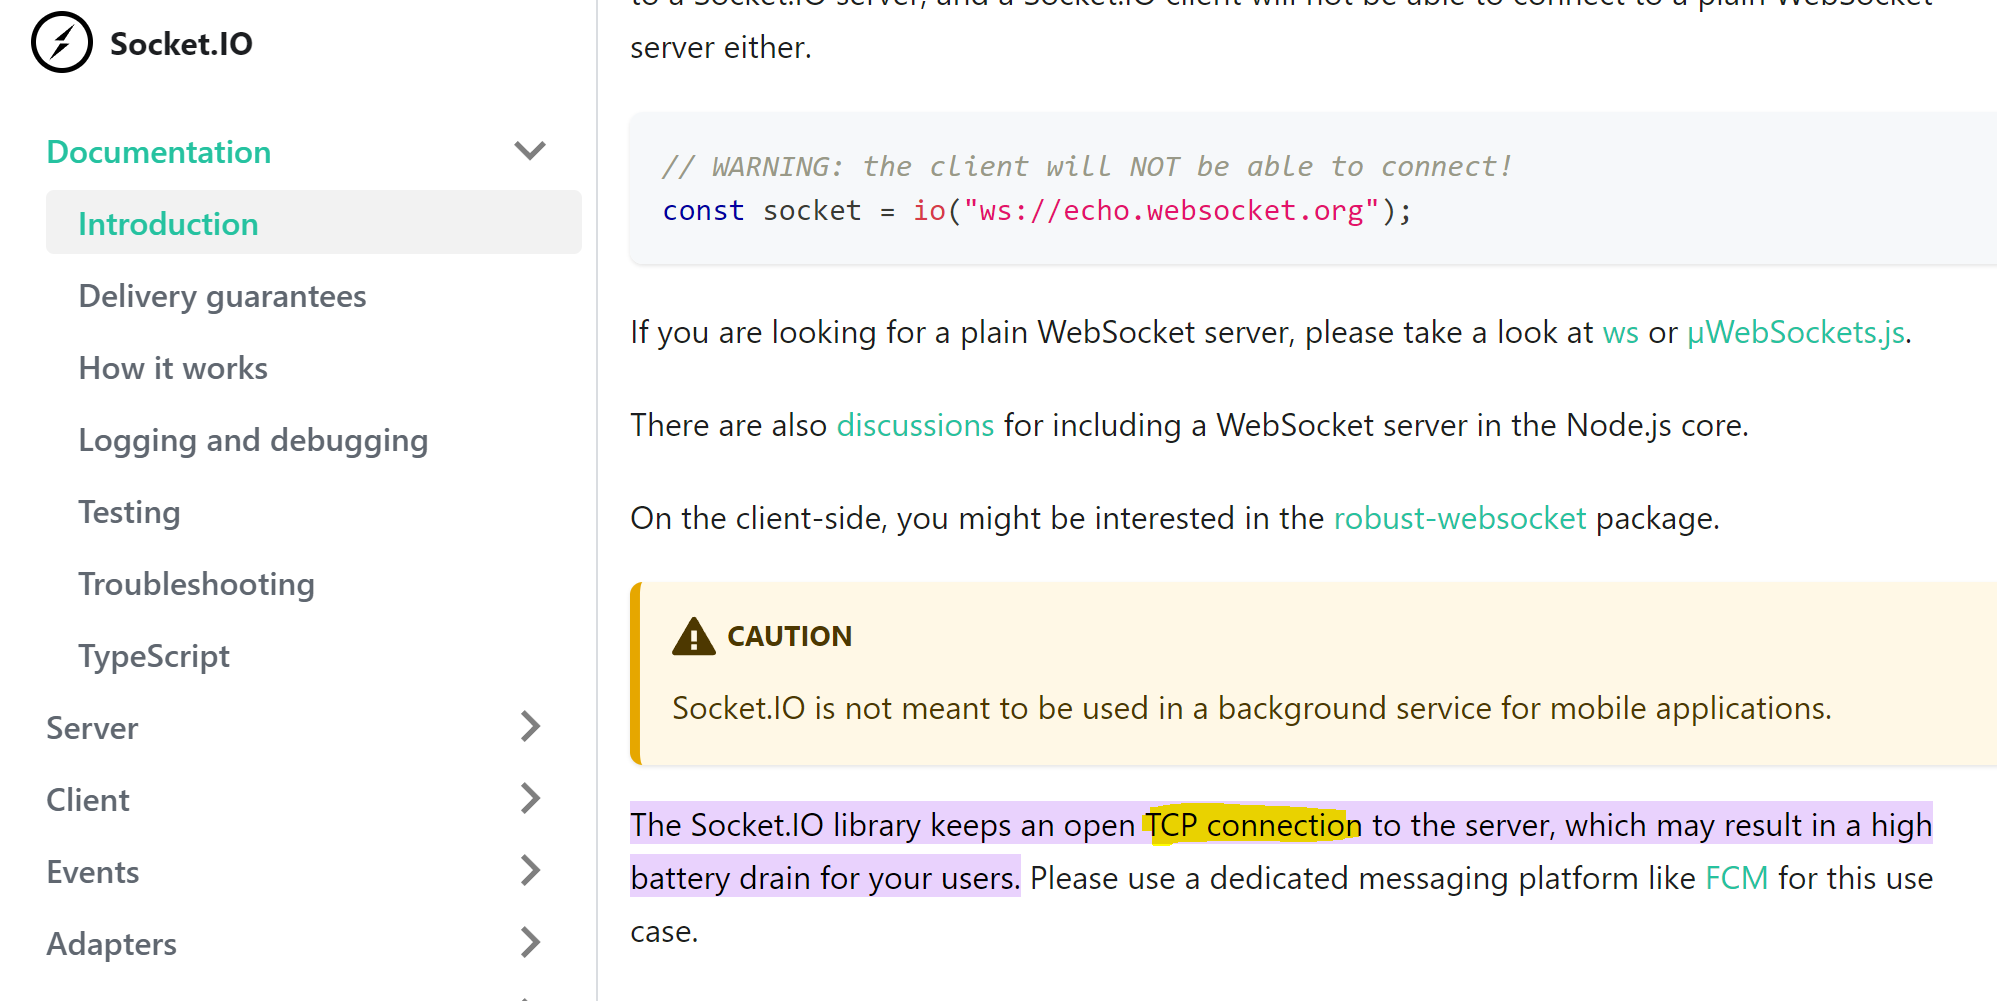
\includegraphics[width=\maxwidth{50.17561465127948em}]{image_3}
\end{flushleft}
\end{par}


\matlabtitle{Q6A}

\matlabheading{Unfortunately my MATLAB is having some trouble downloading the toolbox, so I used QT Framework instead and created the TCP Client and Server implementation in C++ (just as how it should be done in MATLAB). }

\begin{par}
\begin{flushleft}
The port I used will be 5000. The message is sent in UTF-8 encoding. 
\end{flushleft}
\end{par}

\matlabheading{TCP Server Setup:}

\begin{par}
\begin{flushleft}
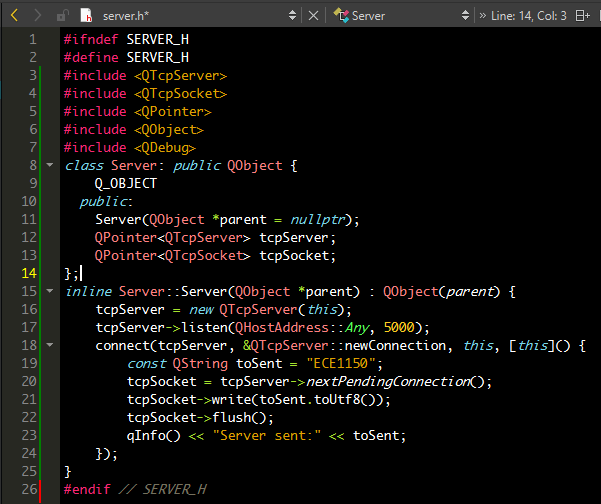
\includegraphics[width=\maxwidth{50.17561465127948em}]{image_4}
\end{flushleft}
\end{par}

\matlabheading{TCP Server Terminal Output:}

\begin{par}
\begin{flushleft}
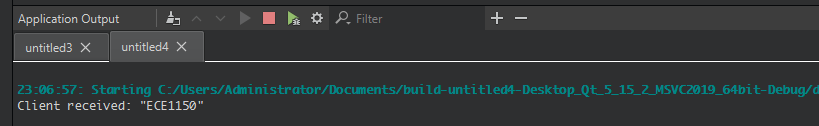
\includegraphics[width=\maxwidth{50.17561465127948em}]{image_5}
\end{flushleft}
\end{par}

\matlabheading{TCP Client:}

\begin{par}
\begin{flushleft}
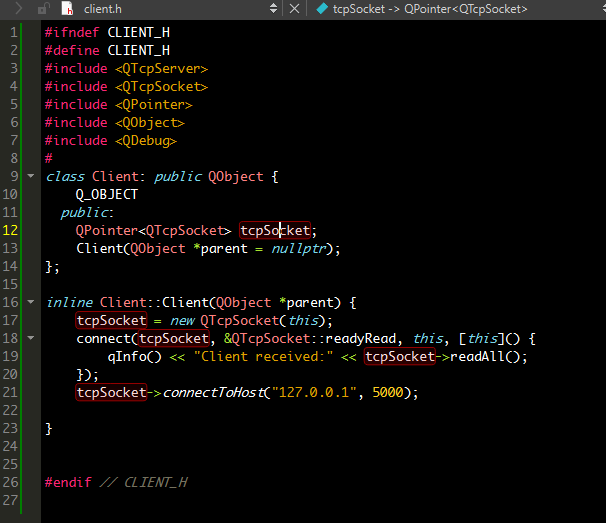
\includegraphics[width=\maxwidth{50.17561465127948em}]{image_6}
\end{flushleft}
\end{par}

\matlabheading{TCP Client Terminal Output:}

\begin{par}
\begin{flushleft}
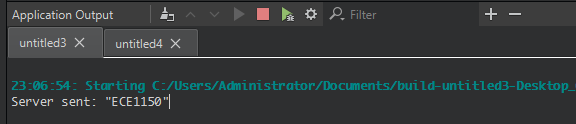
\includegraphics[width=\maxwidth{50.17561465127948em}]{image_7}
\end{flushleft}
\end{par}

\matlabtitle{Q6B}

\begin{par}
\begin{flushleft}
The first three packets are the three-way handshakes. It is used to ensure the connection has been established correctly in TCP protocol. 
\end{flushleft}
\end{par}

\begin{par}
\begin{flushleft}
First packet: The sender generates a random initial sequence number (ISN) and sends it to destination.
\end{flushleft}
\end{par}

\begin{par}
\begin{flushleft}
Second packet: Destination generates a random initial sequence number and sends it along with the acknowledgment to sender.
\end{flushleft}
\end{par}

\begin{par}
\begin{flushleft}
Third packet: Sender acknowledge.
\end{flushleft}
\end{par}

\matlabtitle{Q6C}

\begin{par}
\begin{flushleft}
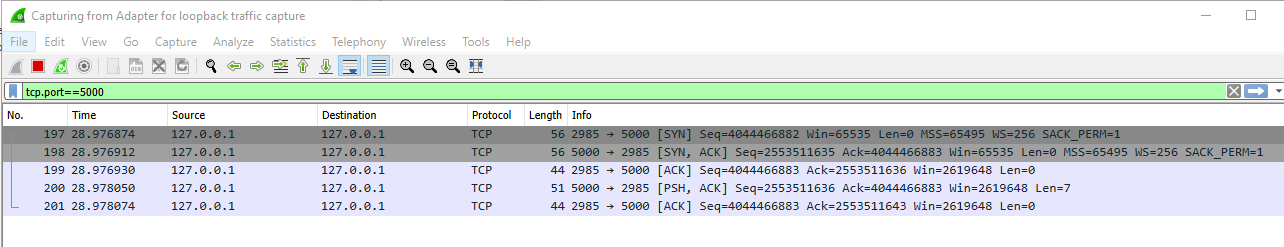
\includegraphics[width=\maxwidth{50.17561465127948em}]{image_8}
\end{flushleft}
\end{par}

\matlabtitle{Q6D}

\begin{par}
\begin{flushleft}
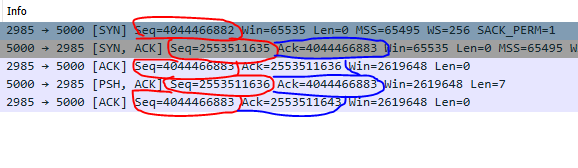
\includegraphics[width=\maxwidth{50.17561465127948em}]{image_9}
\end{flushleft}
\end{par}

\matlabtitle{Q6E}

\begin{par}
\begin{flushleft}
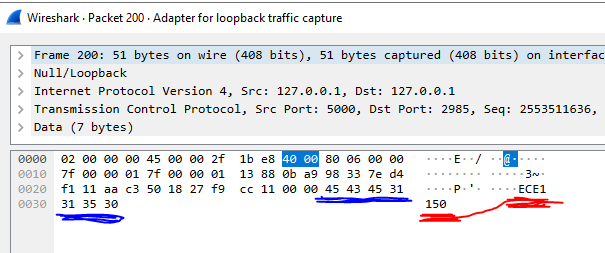
\includegraphics[width=\maxwidth{50.17561465127948em}]{image_10}
\end{flushleft}
\end{par}


\matlabtitle{Q7A}

\begin{par}
\begin{flushleft}
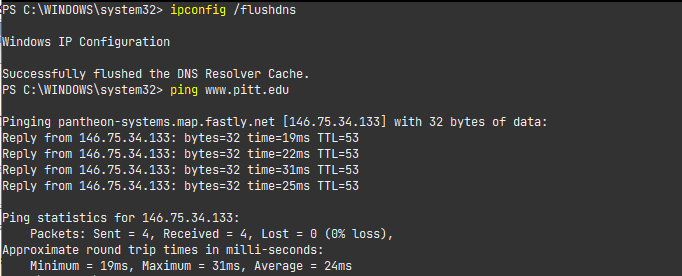
\includegraphics[width=\maxwidth{50.17561465127948em}]{image_11}
\end{flushleft}
\end{par}

\begin{par}
\begin{flushleft}
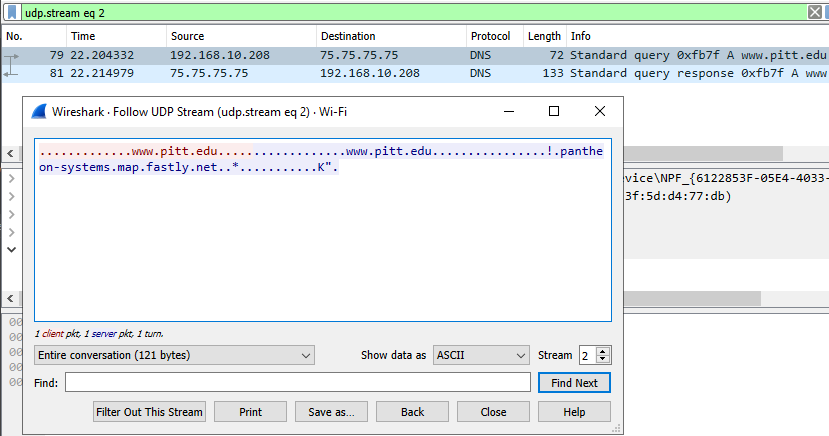
\includegraphics[width=\maxwidth{50.17561465127948em}]{image_12}
\end{flushleft}
\end{par}

\matlabtitle{Q7B}

\begin{par}
\begin{flushleft}
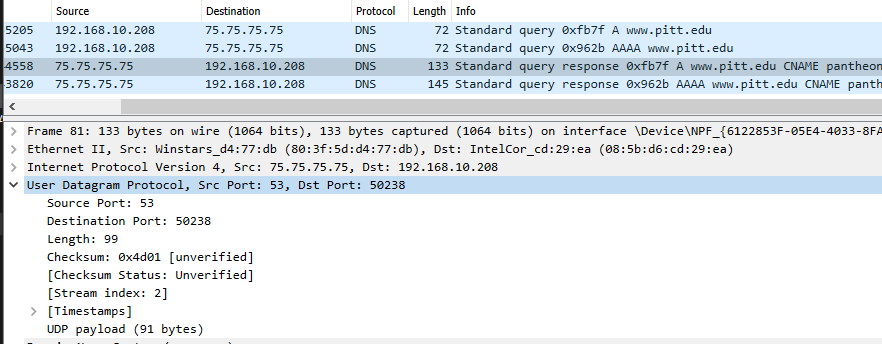
\includegraphics[width=\maxwidth{50.17561465127948em}]{image_13}
\end{flushleft}
\end{par}

\begin{par}
\begin{flushleft}
It is sent over UDP protocol.
\end{flushleft}
\end{par}

\matlabtitle{Q7C}

\matlabheading{Query Message:}

\begin{par}
\begin{flushleft}
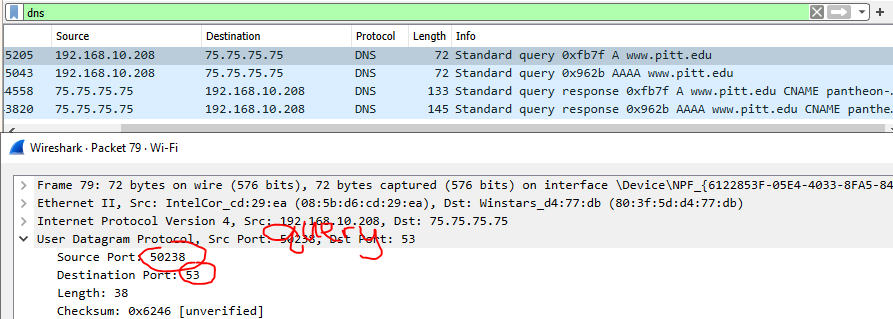
\includegraphics[width=\maxwidth{50.17561465127948em}]{image_14}
\end{flushleft}
\end{par}

\begin{par}
\begin{flushleft}
Source Port : 50238
\end{flushleft}
\end{par}

\begin{par}
\begin{flushleft}
Destination Port: 53
\end{flushleft}
\end{par}

\matlabheading{Response Message:}

\matlabheadingtwo{From the picture in Q7B, we are able to tell:}

\begin{par}
\begin{flushleft}
Source Port: 53
\end{flushleft}
\end{par}

\begin{par}
\begin{flushleft}
Destination Port:  50238
\end{flushleft}
\end{par}

\matlabtitle{Q7D}

\begin{par}
\begin{flushleft}
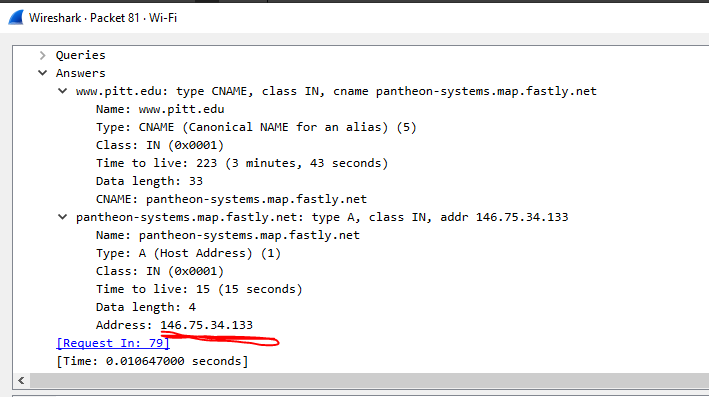
\includegraphics[width=\maxwidth{50.17561465127948em}]{image_15}
\end{flushleft}
\end{par}

\begin{par}
\begin{flushleft}
It is 146.75.34.133.
\end{flushleft}
\end{par}

\matlabtitle{END OF HOMEWORK}

\begin{par}
\begin{flushleft}
The remaining contents are function definitions used mainly in Question 2.
\end{flushleft}
\end{par}


\begin{matlabcode}
function [addr,nBit] = generateForwardingTable (arg1_cA,arg2_cA)
%for q2
arg1_cA = strrep(arg1_cA,' ','');
arg2_cA = strrep(arg2_cA,' ','');
assert(numel(arg1_cA)==numel(arg2_cA));
nBit = find(arg1_cA~=arg2_cA, 1, 'first' )-1;
puts(getEmphCharArray(arg1_cA,1:nBit),'from');
puts(getEmphCharArray(arg2_cA,1:nBit),'to');
% final_cA = bin2dec(reshape(arg1_cA,8,[])')
final_cA = cat(2,arg1_cA(1:nBit),repmat('0',1,32-nBit));
puts(getEmphCharArray(final_cA,1:nBit),'table');
addr = bin2dec(reshape(final_cA,8,[])')';
puts(sprintf("%i.%i.%i.%i | %i", ...
    addr(1),addr(2),addr(3),addr(4),nBit),'res');
end

function [res] = getEmphCharArray (arg1_cA,ind_dA)
res = "";
for i = 1:1:numel(arg1_cA)
    if(ind_dA(1)<=i&&i<=ind_dA(end))
        res = res+sprintf("<strong>%c</strong>",arg1_cA(i));
    else
        res = res+sprintf("%c",arg1_cA(i));
    end
end
end

function [] = puts(arg1_cA,arg2_cA)
fprintf("<strong>%-5s</strong> -> %s\n",upper(arg2_cA),arg1_cA);
end
\end{matlabcode}

\end{document}
